\chapter{Phase-Space Analysis: Two Dimensions}
\label{ch:phase-plane-2d}

\textit{Oscillation requires at least two state variables. This chapter introduces the geometric toolkit for two-dimensional dynamics: vector fields, nullclines, Jacobians, and limit cycles.}

% ============================================================
\section{Two-Dimensional Systems}
\label{sec:2d-systems}
% ============================================================

A two-dimensional dynamical system has the form
%
\begin{equation}
  \dot{x} = f(x, y), \qquad \dot{y} = g(x, y)
  \label{eq:2d-system}
\end{equation}
%
The state of the system is a point $(x, y)$ in the \emph{phase plane}\index{phase plane}. At each point, the functions $f$ and $g$ define a velocity vector $(\dot{x}, \dot{y})$---the direction and speed the state moves. The collection of all these vectors is the \emph{vector field}\index{vector field}. A trajectory is a curve that follows the vector field from some initial condition.

For neuron models, the two variables are typically $V$ (membrane voltage) and a recovery variable---often a potassium gating variable $n$ or a generic slow variable $w$ that provides negative feedback. The voltage is fast (it changes quickly); the recovery variable is slow (it changes on a longer timescale). This separation of timescales is what makes neuroscience models amenable to phase-plane analysis.

% ============================================================
\section{Nullclines}
\label{sec:nullclines}
% ============================================================

A \emph{nullcline}\index{nullcline} is a curve in the phase plane where one of the derivatives vanishes:
%
\begin{equation}
  \text{$x$-nullcline:}\quad f(x, y) = 0, \qquad
  \text{$y$-nullcline:}\quad g(x, y) = 0
  \label{eq:nullclines}
\end{equation}
%
On the $x$-nullcline, $\dot{x} = 0$, so the vector field is purely vertical (the state moves only in the $y$ direction). On the $y$-nullcline, $\dot{y} = 0$, so the vector field is purely horizontal. Where the two nullclines intersect, both derivatives are zero: these are the \emph{fixed points} of the system.

Nullclines are the skeleton of the phase portrait. Once you draw them, you can determine the direction of the vector field in each region by checking the signs of $f$ and $g$. This lets you sketch the qualitative flow without solving a single equation.

For a neuron model with voltage $V$ and recovery variable $n$, the $V$-nullcline is often a cubic-shaped curve (reflecting the N-shape of the total current as a function of voltage), while the $n$-nullcline is a monotonically increasing function (higher voltage means larger steady-state activation). Their intersections determine how many fixed points exist and how the system behaves.

% ============================================================
\section{Fixed Point Classification}
\label{sec:fp-classification}
% ============================================================

Near a fixed point $(x^*, y^*)$, we linearize by setting $(x, y) = (x^*, y^*) + (\delta x, \delta y)$:
%
\begin{equation}
  \begin{pmatrix} \dot{\delta x} \\ \dot{\delta y} \end{pmatrix}
  \approx J \begin{pmatrix} \delta x \\ \delta y \end{pmatrix},
  \qquad
  J = \begin{pmatrix}
    \partial f/\partial x & \partial f/\partial y \\
    \partial g/\partial x & \partial g/\partial y
  \end{pmatrix}_{\!(x^*,\, y^*)}
  \label{eq:jacobian}
\end{equation}

The eigenvalues of the Jacobian\index{Jacobian} $J$ determine the local geometry. The characteristic equation is $\lambda^2 - \tau\lambda + \Delta = 0$, where $\tau = \tr(J)$ and $\Delta = \det(J)$.

\begin{keyequation}[Trace--Determinant Classification]
\begin{equation}
  \lambda_{1,2} = \frac{\tau \pm \sqrt{\tau^2 - 4\Delta}}{2}
  \label{eq:eigenvalues}
\end{equation}
\tcblower
$\tau = \tr(J)$: controls stability (negative $\to$ stable). \quad
$\Delta = \det(J)$: sign distinguishes saddles from nodes/spirals. \\[4pt]
$\tau^2 - 4\Delta$: sign distinguishes nodes (real $\lambda$) from spirals (complex $\lambda$).
\end{keyequation}

\noindent The classification is as follows. If $\Delta < 0$, the eigenvalues are real with opposite signs: the fixed point is a \emph{saddle}\index{saddle point}. If $\Delta > 0$ and $\tau < 0$, both eigenvalues have negative real parts: the fixed point is a \emph{stable node} (real eigenvalues) or \emph{stable spiral} (complex eigenvalues, meaning damped oscillations). If $\Delta > 0$ and $\tau > 0$, the fixed point is an unstable node or spiral. The boundary $\tau^2 = 4\Delta$ separates nodes from spirals.

\subsection{Why saddles matter for neurons}

Saddle points\index{saddle point} appear frequently in neuron models, and they play a disproportionately important role. A saddle has one attracting direction and one repelling direction. The \emph{stable manifold}\index{stable manifold} of a saddle---the curve along which trajectories approach it---acts as a separatrix, dividing the phase plane into qualitatively different regions. In neuron models, this separatrix is the geometric object behind ``threshold'': trajectories on one side return to rest, trajectories on the other side produce a spike.

This is a much richer picture of threshold than the one-dimensional version. In two dimensions, threshold is not a single voltage value---it is a \emph{curve} in the $(V, n)$ plane. A stimulus that brings the state across this curve triggers a spike; one that does not, no matter how close, does not.

% ============================================================
\section{Limit Cycles}
\label{sec:limit-cycles}
% ============================================================

A \emph{limit cycle}\index{limit cycle} is a closed trajectory in the phase plane: the state returns to its starting point after a period $T$, and the motion repeats indefinitely. A \emph{stable} limit cycle attracts nearby trajectories: if the state starts near the cycle, it spirals onto it. A stable limit cycle is the mathematical object behind repetitive spiking---each orbit around the cycle corresponds to one action potential.

Limit cycles cannot exist in one dimension (trajectories on a line cannot return to their starting point without stopping at a fixed point in between). They are an essentially two-dimensional phenomenon.

As a parameter (say, the injected current) increases, a stable fixed point can lose stability and give way to a limit cycle. The specific way this transition happens---the \emph{bifurcation}\index{bifurcation}---determines the neuron's excitability type, which is the subject of \cref{ch:excitability}.

% ============================================================
\section{A Worked Example: The Persistent Sodium Model in 2D}
\label{sec:persistent-na-2d}
% ============================================================

To make these ideas concrete, consider a two-variable reduction of the Hodgkin--Huxley model with persistent sodium and potassium:
%
\begin{align}
  \Cm\dot{V} &= -\gbar{Na}\,\minf(V)\,(V - \Erev{Na}) - \gbar{K}\,n\,(V - \Erev{K}) - \gleak(V - \Erev{L}) + I_{\text{ext}} \label{eq:2d-V} \\[4pt]
  \dot{n} &= \frac{\ninf(V) - n}{\tau_n(V)} \label{eq:2d-n}
\end{align}
%
The $V$-nullcline ($\dot{V} = 0$) is the curve $n = n_V(V)$ obtained by solving the right-hand side of \cref{eq:2d-V} for $n$. It is typically cubic-shaped: an N-curve with a left branch (rest), a middle branch (unstable), and a right branch (excited). The $n$-nullcline ($\dot{n} = 0$) is $n = \ninf(V)$, which is a monotone sigmoid.

Their intersection gives the fixed points. When the current $I_{\text{ext}}$ is small, the intersection is on the left branch---a stable resting state. As current increases, the $V$-nullcline shifts (current pushes the curve up), and the fixed point moves along the nullcline. Beyond a critical current, the fixed point can lose stability and a limit cycle appears---the neuron fires repetitively.

The full action potential trajectory traces a large loop in the $(V, n)$ plane: rapid depolarization (fast $V$ increase with $n$ lagging behind), followed by repolarization (increasing $n$ opens potassium channels), afterhyperpolarization (high $n$, low $V$), and recovery ($n$ slowly decreases back to baseline). The nullclines organize this loop.

\begin{figure}[h]
\centering
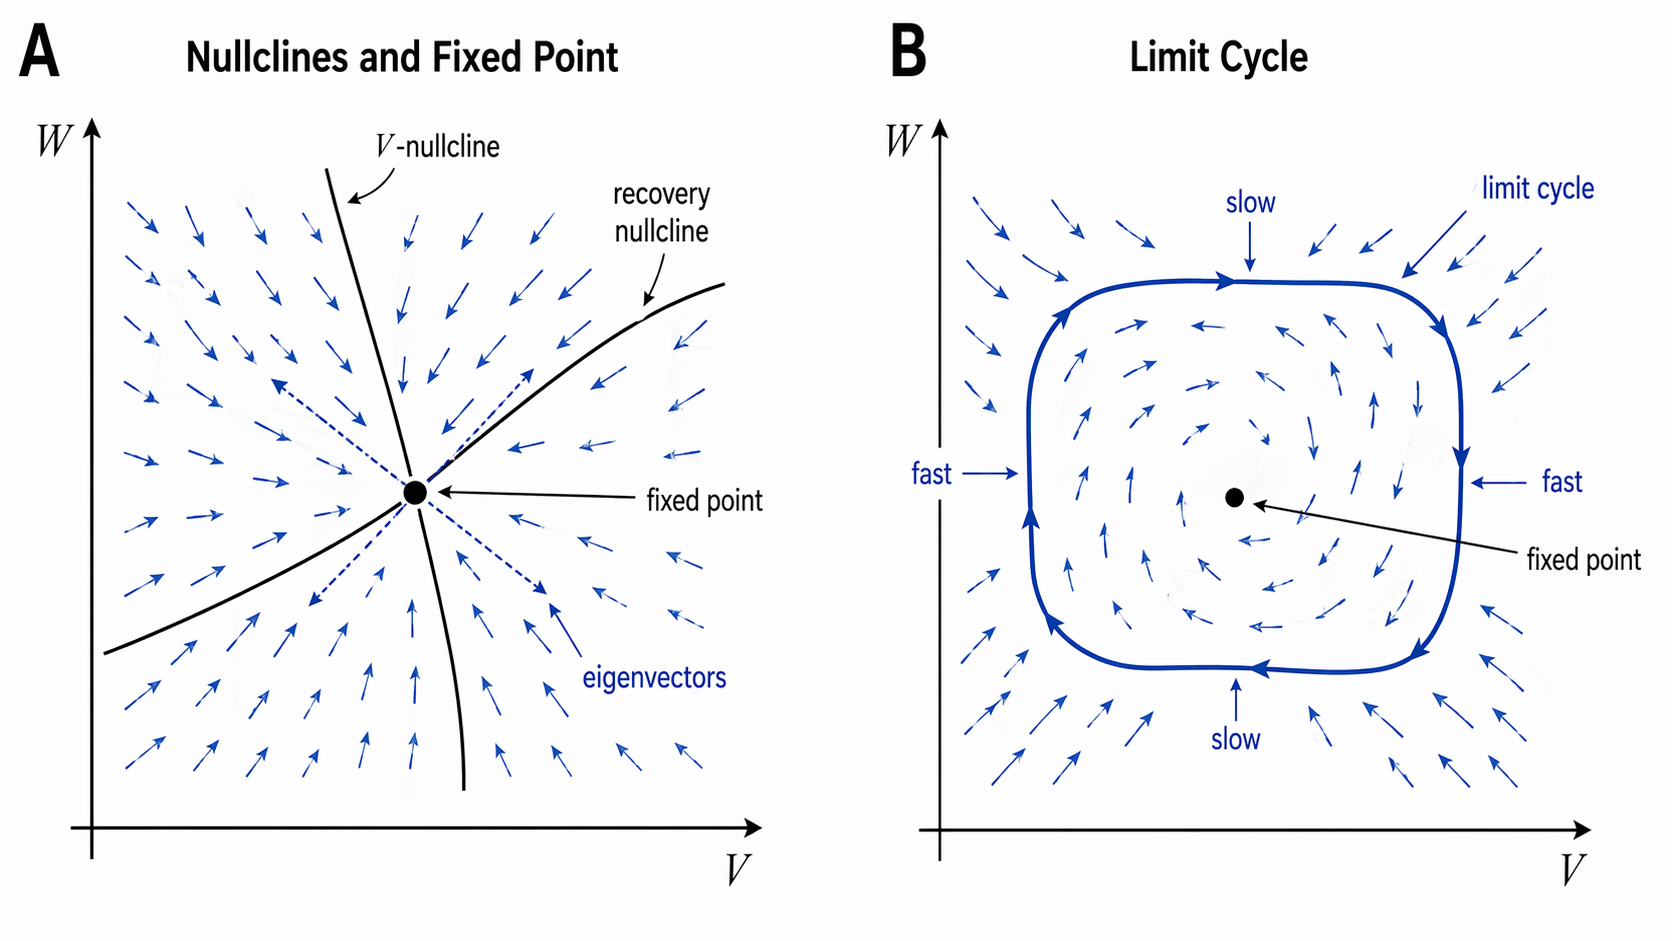
\includegraphics[width=\textwidth]{figures/mns-2d-phase-plane.png}
\caption{Two-dimensional phase geometry. Nullcline intersections locate fixed points and the vector field gives local motion; repetitive spiking corresponds to an attracting limit cycle in the voltage--recovery plane.}
\label{fig:phase-plane-2d}
\end{figure}


\begin{chaptersummary}

\begin{center}
\renewcommand{\arraystretch}{1.6}
\begin{tabularx}{\textwidth}{@{}l X X@{}}
  \toprule
  \textbf{Concept} & \textbf{Equation} & \textbf{Key Insight} \\
  \midrule
  2D system &
  $\dot{x} = f(x,y)$, $\dot{y} = g(x,y)$ &
  Trajectories in phase plane \\
  %
  Nullclines &
  $f = 0$, $g = 0$ &
  Skeleton of the flow; intersections $=$ FPs \\
  %
  Jacobian &
  $\displaystyle J = \begin{pmatrix} f_x & f_y \\ g_x & g_y \end{pmatrix}$ &
  Eigenvalues classify local dynamics \\
  %
  Trace--det &
  $\Delta < 0$: saddle; $\tau < 0$: stable &
  Quick classification without computing $\lambda$ \\
  %
  Limit cycle &
  Closed orbit, period $T$ &
  Repetitive spiking = stable limit cycle \\
  \bottomrule
\end{tabularx}
\end{center}

\end{chaptersummary}

\begin{conceptquestions}
  \item Why can oscillations exist in two dimensions but not in one? What geometric property of trajectories in 2D makes this possible?

  \item You are given the nullclines of a 2D neuron model. Without computing anything, how can you determine the direction of the vector field in each region of the phase plane?

  \item Explain why nullcline intersections are fixed points. If two nullclines intersect three times, what can you say about the stability of the three fixed points?

  \item The Jacobian matrix $J$ evaluated at a fixed point has trace $\tau$ and determinant $\Delta$. Explain the physical meaning of each: what does $\tau$ control, and what does $\Delta$ control?

  \item A fixed point has complex eigenvalues with negative real part. Describe the trajectory of a perturbation near this fixed point. How does the behavior change if the real part becomes positive?

  \item A saddle point's stable manifold acts as a separatrix in neuron models. Why is this a more accurate description of ``threshold'' than a single voltage value? How does the separatrix relate to the concept of threshold in the one-dimensional analysis of \cref{ch:phase-plane-1d}?

  \item In the persistent sodium model, the $V$-nullcline is cubic-shaped. What happens to the fixed point as $I_{\text{ext}}$ increases? Describe the sequence of qualitative changes.

  \item A limit cycle is a closed orbit in the phase plane. What is the difference between a stable and an unstable limit cycle? How do nearby trajectories behave in each case?

  \item The $V$-nullcline of a typical neuron model has a cubic (N-shaped) form. Explain why: what biophysical features of the voltage equation produce the left branch, the middle branch, and the right branch?

  \item In the 2D persistent sodium model, trace the action potential trajectory in the $(V, n)$ plane. Why does the trajectory form a large loop rather than returning along the same path? What role does the separation of timescales play?

  \item Two neurons can have identical nullclines but different timescale separations (one has $\tau_n$ much larger than the other). How does the timescale ratio affect the shape of the action potential in the phase plane?

  \item Explain why increasing $I_{\text{ext}}$ shifts the $V$-nullcline but not the $n$-nullcline. What does this tell you about how external input changes the number and location of fixed points?

  \item Can a 2D system have more than one stable limit cycle? Can a stable limit cycle and a stable fixed point coexist? What does this imply for the neuron's response to stimuli of different strengths?
\end{conceptquestions}
